\chapter{Entwurf}
\section{Projektverwaltung und Werkzeuge}
In diesem Abschnitt wird die interne Projektverwaltung, die Werkzeuge zur Projektverwaltung und die Werkzeuge zur Projektrealisierung beschrieben.
Die Aufgabenstellung und der Fortschritt des Projekts wurde fortlaufen in Treffen mit \textit{Herrn Professor Teßmann} besprochen. Zwischen den Treffen stand \textit{Herr Professor Teßmann} jederzeit für persönliche und schriftliche Fragen zur Verfügung.

\subsection{GitHub}
Zur kollaborativen Versionsverwaltung wird der Online-Service \textbf{GitHub} verwendet, welcher für OpenSource Projekte kostenlos öffentliche Repositories zur Verfügung stellt. Da das Projekt unter der \textbf{MIT-Lizenz} entwickelt wird, ist die Nutzung eines öffentlichen Repositories ein Vorteil hinsichtlich auf eine mögliche Weiterentwicklung und einer guten Akzeptanz in der OpenSource-Community.

Das GitHub-Repository bietet die Möglichkeit den Code, welcher lokal entwickelt wird, in das Repository hochzuladen, so dass immer ein konsistenter gleicher Versionsstand vorhanden ist. Außerdem gibt es die Möglichkeit für einzelne Teilprojekte eigene \textbf{Branches} zu erstellen, so dass auf diesen unabhängig vom Master-Branch, in welchem alle Teile zusammenfließen, entwickelt werden kann.

Zur Fehlerverwaltung wird das bereits Integrierte \textbf{Issue System} von GitHub verwendet. Mit diesem ist es möglich die Issues zu priorisieren, mit Tags zu versehen, einzelnen Projektmitgliedern zuzuweisen und den Bearbeitungsstand zu dokumentieren. Der weitere Vorteil hiervon ist, das jedes Projektmitglied automatisch eine Benachrichtigung über neue Issues und Aktualisierungen erhält und somit bei der Fehleranalyse helfen kann.
Außerdem wurden einzelne \textbf{Milestones} erstellt, welche sich an den fortlaufenden Besprechungen orientierten und somit laufend Ziele bei der Projektdurchführung definierten. Nach der Erreichung großer Projektziele wurden Versionsstände als \textbf{Releases} getaggt, so dass ersichtlich wurde, welchen funktionellen Umfang der Code in diesem Stadium hat.

\subsection{CMake}
Da das Ziel \ref{NFA:Plattformunabhängigkeit} des Projektes ist, plattformunabhängig zu sein, wird eine Möglichkeit benötigt unterschiedliche \textbf{integrierte Entwicklungsumgebungen (IDEs)} zu unterstützen.
Hierfür wurde das plattformunabhängige Build Werkzeug CMake, welches auch unter einer OpenSource Lizenz (BSD-Lizenz) erhältlich ist, verwendet. CMake erlaubt es für unterschiedliche IDEs Projektdateien zu erstellen, so dass für die Entwicklung nicht eine spezifische Entwicklungsumgebung benötigt wird, sondern mit mehreren, auch betriebssystemunabhängigen IDEs, entwickelt werden kann.

\subsection{IDEs}
Als IDEs kamen \textbf{Visual Studio} unter Windows 7 und Windows 10 zum Einsatz. Zu Beginn des Projekts in Version Visual Studio 2013, in der zweiten Hälfte des Projekts dann in Version Visual Studio 2015, welches eine bessere Unterstützung für C++11 Sprachfeatures enthält. Unter Fedora 21 wurde \textbf{Netbeans} in Version 8 eingesetzt.

\subsection{Testumgebung}
Zum Testen des Codes wurden mehrere unterschiedliche Testumgebungen eingesetzt. Dabei wurden \textbf{rechnerübergreifende Tests} des Verbindungsaufbaus und der Verbindungsqualität über \textit{LAN}, \textit{WLAN} und \textit{WAN} mit verschiedenen Betriebssystemen durchgeführt. 

Zum Testen einzelner Module des Projektes wurde die Unit-Test Umgebung \textbf{CPPTest} eingesetzt, die es ermöglicht einzelne Module auf ihre funktionalen Anforderungen hin zu überprüfen. 

Für einen automatisierten Build-Test wurde auf den Online-Service \textbf{Travis CI} gesetzt, der durch seine einfache Integration in das GitHub Repository eine gute Lösung bietet. Er bietet die Möglichkeit, schnell herauszufinden, ob der neu eingecheckte Code fehlerfrei unter \textit{Linux} und \textit{OSX} kompiliert.

\section{Build Prozess}
\subsection{CMake}
Die CMake Konfiguration basiert auf mehreren \texttt{CMakeLists.txt}-Dateien, welche \textbf{hierarchisch} in die Projektstruktur integriert sind. In der Konfigurationsdatei auf der obersten Ebene wird die minimal benötigte CMake \textit{Version} und der \textit{Projektname} definiert.
Außerdem werden IDE abhängige Einstellungen vorgenommen wie z.B. die Einstellung des \textit{Warning Levels} für Compilefehler und die Unterstützung von \textit{Unicode} Zeichen unter Visual Studio.
Anschließend werden die relativen Pfade, in welche die fertig kompilierten Dateien abgelegt werden, definiert und die unteren Ordnerstrukturen mit ihren dort befindlichen Konfigurationsdateien angegeben.

In diesen weiteren Konfigurationsdateien für \textbf{OHMComm} und den extern benutzten Softwarekomponenten wie \textbf{Rtaudio} und \textbf{Opus} wird nun festgelegt, welche \textit{Header} und welche \textit{C++ Dateien} eingebunden werden. 

\subsection{Build unter Unix}
Zum Erstellen des Projektes OHMComm unter Unix-Systemen wird neben einem C++11-fähigen Compiler und dem Programm \textbf{CMake} noch die \textbf{Make} Build-Suite sowie eine Audio-Bibliothek mitsamt Header-Dateien benötigt. Während Make und eine Audio-Bibliothek auf den meisten Unix-Systemen bereits mitgeliefert werden, müssen die Entwicklungs-Header für die verwendete Audio-Bibliothek meist erst noch installiert werden. Als Audio-Bibliothek wird unter Linux-Systemen OSS, ALSA, Jack und PulseAudio unterstützt \cite{RTAudioAPIs}. Die Entwicklungs-Header für die Audio-Bibliotheken liegen je nach System -- oder genauer: je nach Paketverwaltungssystem -- in verschieden benannten Paketen. So heißt das Paket für die ALSA-Header unter Debian \texttt{libasound-dev} und unter Fedora \texttt{alsa-lib-devel}.
Unter Linux und den meisten Unix-Betriebssystemen wird das Projekt kompiliert, indem zuerst mit dem Befehl \texttt{cmake -G ``Unix Makefiles''} aus der CMake-Beschreibung eine \texttt{Makefile} -- also eine Anleitung für das \texttt{make} Build-System -- erstellt wird. Daraufhin können mit dem Befehl \texttt{make} im Zielverzeichnis des vorherigen Kommandos die einzelnen Bibliotheken oder Programme kompiliert werden. So erstellt \texttt{make OHMCommLib} die Bibliothek \textbf{OHmCommLib} (das eigentliche Framework), die in weitere Programme eingebunden werden kann (siehe Abschnitt \ref{configurationUsages}). \texttt{make OHMComm} erstellt das ausführbare Programm \textbf{OHMComm} (siehe Ziel \ref{FA:Konsolenanwendung}) und \texttt{make Tests} die Test-Suite für das Projekt.

\subsection{Build unter Windows}
Zum Erstellen des Projekts unter Windows wird eine aktuelle Version von \textbf{CMake} und die zu benutzende \textbf{Entwicklungsumgebung}, welche von CMake unterstützt wird, benötigt.
Für einen sauberen Entwicklungsprozess ist es zu empfehlen, sich ein Build Verzeichnis außerhalb des Sourcecodes anzulegen (Out-of-Source Build).

\begin{figure}[htp]
\centering
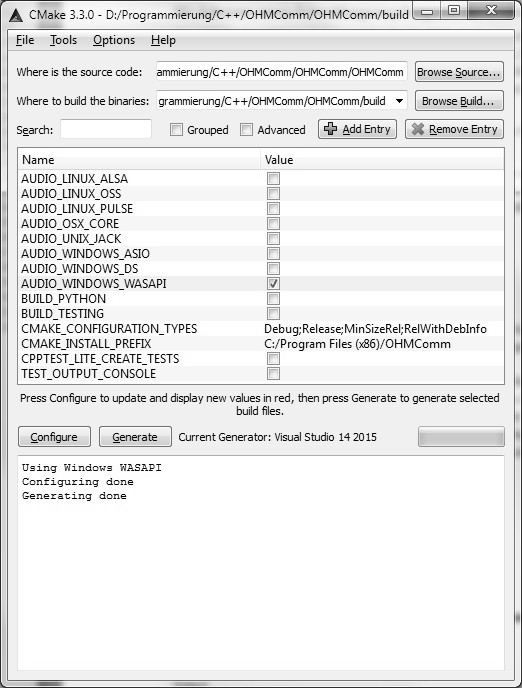
\includegraphics[width=.80\textwidth]{images/CMake}
\caption{CMake Konfiguration unter Windows 7}
\label{Fig:CMake}
\end{figure}

Es wird CMake mitgeteilt wo sich der Source Code (\texttt{Browse Source}) und das Build Verzeichnis (\texttt{Browse Build}) befindet.
Mittels \texttt{Configure} wird der Compiler und die verwendete Entwicklungsumgebung definiert.
Anschließend wird ausgewählt welche Audio Bibliothek verwendet wird, unter Windows wird \textit{ASIO}, \textit{DS} und \textit{WASAPI} unterstützt. Wahlweise kann auch \textit{CppTest} aktiviert werden, falls die Tests erstellt werden sollen.
Die Einstellungen werden durch nochmaligen Druck auf \texttt{Configure} bestätigt und über \texttt{Generate} werden die Projektdateien im vorher definierten Buildverzeichnis erstellt.

Es wird die \textit{Entwicklungsumgebung} mit den generierten Projekt Dateien gestartet und angewiesen das Projekt zu kompilieren.

Im Verzeichnis \texttt{build/Release/} findet sich bei der Verwendung von Visual Studio und Kompilierung mit Release Optionen das ausführbare Programm \textbf{OHMComm.exe} und die OHMComm Bibliothek \textbf{OHMComm.lib}.

\section{Softwarearchitektur}
\subsection{Konfiguration und Verwendung}
\label{configurationUsages}
Um OHMComm verwenden zu können, müssen vorher eine Vielzahl an Einstellungen getroffen werden. Diese Einstellungen gliedern sich in folgende Bereiche:
\begin{description}
\item[Audio-Konfiguration:]Einstellungen für die Soundkarte, wie die Wahl des Formats zum Aufnehmen oder Abspielen, die Anzahl der Kanäle, die Abtastrate oder die verwendeten Audiogeräte. Die Auswahl der Geräte für die Aufnahme und Ausgabe können unabhängig vom Kommunikationspartner eingestellt werden. Andere Einstellungen (Audioformat, Kanäle und Abtastrate) müssen jedoch mit dem Gesprächspartner abgestimmt oder auf kompatible Werte umgerechnet werden.
\item[Prozessoren-Konfiguration:]Hierunter fällt die Auswahl der verwendeten Audioprozessoren und die Reihenfolge, in der die Prozessoren verkettet werden (siehe Abschnitt \ref{processingChain}). Ebenso besitzen manche Prozessoren eigene Einstellungsmöglichkeiten, um deren Funktionsweise zu regeln. Die meisten Prozessoren und -Einstellungen fordern keine Anpassung der Konfiguration des Gesprächspartners. Ausnahmen sind hier die Audiocodecs, die von beiden Programmen gleich konfiguriert verwendet werden müssen, um die encodierten Daten wieder richtig decodieren zu können.
\item[Netzwerk-Konfiguration:]Bestimmt den zu verwendeten Port zum Empfangen und Senden von Paketen auf dem lokalen Rechner, sowie die IP-Adresse und den Port des Rechners des Kommunikationspartners. Die Ports und die Adresse des jeweils anderen Rechners müssen vorher zwischen den Gesprächspartner abgestimmt werden, um eine Duplex-Kommunikation einrichten zu können. Bei der Netzwerk-Konfiguration ist zu beachten, dass bei Kommunikation über ein WAN (Wide Area Network) eine von außen erreichbare IP-Adresse gewählt wird evtl. auch Port-Weiterleitungen eingerichtet werden müssen.
\item[Sonstige Konfiguration:] Hier zählen sonstige, rein optionale Einstellungen, die die eigentliche Audiokommunikation nicht beeinflussen, wie das Messen der Ausführungsdauer der verwendeten Prozessoren, das Schreiben des Logs in eine Datei sowie die informativen Daten, die bei RTCP SDES-Paketen gesendet werden (siehe Abschnitt \ref{rtcp}). Da diese Einstellungen nur das lokale Programm betreffen, müssen sie nicht mit dem Gegenüber abgestimmt werden.
\end{description}
Für die meisten nicht-optionalen Einstellungen sind Standardwerte vorgegeben (wie den beiden Ports für den lokalen und entfernten Rechner) oder werden beim Start des Programms ermitteln (wie die Standard-Audiogeräte für die Ein- und Ausgabe). Um die einfachste Form der Kommunikation aufbauen zu können -- ohne Audiocodecs oder sonstigen Audioprozessoren -- muss nur die IP-Adresse des Gegenübers gesetzt werden. jedoch empfiehlt es sich aus verschiedenen Gründen (wie die Reduzierung der Bandbreite) eine erweiterte Konfiguration vorzunehmen.
\\%TODO: nach Steuerung?
OHMComm implementiert eine Vielzahl an Konfigurationsmöglichkeiten, um einen möglichst breiten Verwendungsbereich zu bieten. So kann die prototypische Anwendung aus Kapitel \ref{prototypProgram} als interaktive Konsolen-Anwendung gestartet werden. Dabei werden alle Einstellungsmöglichkeiten nacheinander ausgegeben und der Benutzer kann durch Eingabe einen der vorgeschlagenen Werte auswählen oder einen eigenen Wert eingeben, je nach Art der Einstellung.
\\
Ebenso kann die Konfiguration durch Kommandozeilen-Argumente vorgenommen werden. Hierfür benutzt OHMComm den aus Unix bekannten Syntax, bei dem Schlüssel-Werte Paare mit einem Gleichheitszeichen = getrennt angegeben werden, z.B. \texttt{--local-port=54321} für die Bestimmung des lokalen Ports. Ebenso werden für die meisten Optionen sowohl ein kurzer als auch ein langer Schlüssel unterstützt. So geben beide Argumente \texttt{-h} und \texttt{--help} die Hilfe auf der Kommandozeile aus, die alle verfügbaren Parameter und deren Bedeutung sowie Standard-Werte anzeigt. Die gleichen Parameter können auch aus einer Konfigurationsdatei geladen werden. Dafür werden dort die Schlüssel-Wert Paare zeilenweise und auch durch ein Gleichheitszeichen getrennt (aber ohne führende Bindestriche) aufgelistet und die Datei beim Start an das OHMComm-Programm als einzigen Parameter übergeben.
\\
Um das Programm auch als Bibliothek verwenden zu können, wird eine Möglichkeit geboten, über Methodenaufrufe die benötigten und optionalen Einstellungen zu setzen. %TODO: Verwendung als Bib, Was kanns? Nutzen
\\
Des Weiteren gibt es die sog. \textbf{passive Konfiguration}, bei der alle Konfigurationen, die in beiden Programmen gleich eingestellt sein müssen, vor dem Start der Kommunikation ausgetauscht werden. Zu den ausgetauschten Einstellungen zählen Abtastrate, Audioformat, Anzahl der Kanäle und die verwendeten Prozessoren (für die Audiocodecs). Somit wird die Gleichheit dieser Einstellungen garantiert und der Konfigurationsaufwand verringert. Mehr Informationen zur Umsetzung der passiven Konfiguration finden sich in Abschnitt \ref{passiveConfiguration}.

\subsection{Audio-Schnittstelle}
Für die Audioverarbeitung ist ein allgemeine Schnittstelle zur Audiohardware nötig, siehe Anforderung \ref{FA:SchnittstelleAudiohardware}. Dabei gilt es insbesondere die nicht-funktionalen Anforderungen \ref{NFA:Plattformunabhängigkeit}, \ref{NFA:Performanz} und \ref{NFA:Softwarearchitektur} zu berücksichtigen. Es wird eine abstrakte Klasse mit dem Namen \texttt{AudioHandler} erstellt, welche die Verbindung zur Hardware darstellt. Sämtliche Audiodaten laufen über diese Schnittstelle zum Mikrofon oder zu den Lautsprechern. 

\subsubsection{Verarbeitungsmethoden}
Die Klasse bietet drei virtuelle Methoden, welche eine automatische Verarbeitung starten. Die Methode \texttt{start"-Recording"-Mode()} startet die Verarbeitung von Audioinputdaten (Mikrofon), \texttt{start"-Playback"-Mode()} startet die Verarbeitung von Audiooutputdaten (Lautsprecher) und \texttt{start"-Duplex"-Mode()} ist die gleichzeitige Verarbeitung von Audioinput- und Audioutputdaten. Letztere stellt den Standardfall für die Audiokommunikation dar. Wie diese Methoden im Detail aussehen, wird in Unterklassen von \texttt{AudioHandler} implementiert. Für die Hardwareansteuerung ist es sinnvoll, bereits existierende Lösungen zu verwenden. In diesem Fall kann man Unterklassen von \texttt{AudioHandler} auch als Wrapper-Klassen ansehen.

\subsubsection{Konfiguration}
Vor der Verarbeitung muss die Hardware konfiguriert werden. Hierfür muss das Struct \texttt{AudioConfiguration} verwendet werden. In diesem lassen sich das Mikrofon und die Lautsprecher bestimmen, die Anzahl der Kanäle (Mono - Stereo), die Sample Rate und die Größe des internes Buffers. Der interne Buffer kann vorerst vernachlässigt werden. Im Kapitel von \ref{sec:RTAudio} wird dieser näher erläutert. Für die Übergabe der Einstellungen steht in der Klasse \texttt{AudioHandler} die Methode \texttt{setConfiguration()} zur Verfügung. Falls keine Konfiguration übergeben wird, so wird automatisch die virtuelle Methode \texttt{setDefaultAudioConfig()} aufgerufen. Diese muss ebenfalls von der Unterklasse implementiert werden. Ihre Aufgabe ist es eine Standardkonfiguration zur Verfügung zu stellen, falls die Klasse nicht konfiguriert wurde. Es ist jedoch zu beachten, dass Standardkonfiguration eventuell fehlerhaft und nicht auf allen Systemen lauffähig ist.

\subsubsection{Steuerung der Verarbeitung}
Eine laufende Verarbeitung durch folgende Methoden gesteuert werden: Die Methode \texttt{suspend()} pausiert die aktuelle Verarbeitung und \texttt{resume()} setzt sie weiter fort. Die Methode \texttt{stop()} bricht den gesamten Verarbeitungsvorgang ab, welcher anschließend auch nicht mehr mit \texttt{resume()} fortgesetzt werden kann. \texttt{reset()} ruft intern \texttt{stop()} auf und setzt die übergebene Audiokonfiguration zurück.

\subsubsection{Prepare-Methode}
Die virtuelle Methode \texttt{prepare()} nimmt eine Sonderrolle ein. Grundsätzlich kann Sie als optional betrachtet werden, jedoch ist sie für bestimmte Einsatzzwecke sinnvoll. Sie sollte aufgerufen werden nachdem eine Audiokonfiguration übergeben worden ist, jedoch bevor die Verarbeitung gestartet wird. Dies kann sinnvoll sein um z.B. die ausgewählte Hardware im Hinblick auf bestimmte Einstellungsmöglichkeiten und deren Kompatiblität mit anderen Komponenten zu überprüfen. Falls eine Inkompatiblität festgestellt wird, kann der Start der Verarbeitung abgebrochen werden.

\FloatBarrier
\subsubsection{Fazit}
Abbildung \ref{Fig:AudioHandlerAnySimple} zeigt eine vereinfachte Darstellung des \texttt{AudioHandlers}. Durch die abstrakte Klasse wird gewährleistet, dass die Klasse austauschbar und erweiterbar ist. Viele Implementierungsdetails werden in die Unterklasse ausgelagert. Durch das Verwenden externer Libraries kann die Unterklasse auch als Wrapper-Klasse angesehen werden. Die Audiohardware lässt sich durch das Struct \texttt{Audio"-Configuration} konfigurieren. Jedoch besteht diese Klasse nicht nur aus der Schnittstelle zur Hardware, sondern ist der zentraler Verarbeitungspunkt, daher einer der wichtigsten Komponenten des Frameworks. Für die Verarbeitung von Audiodaten wurde eine spezielle Schnittstelle, die Verarbeitungskette, integriert. Im folgenden Kapitel wird diese näher erläutert.
\newline
\begin{figure}[htp]
\centering
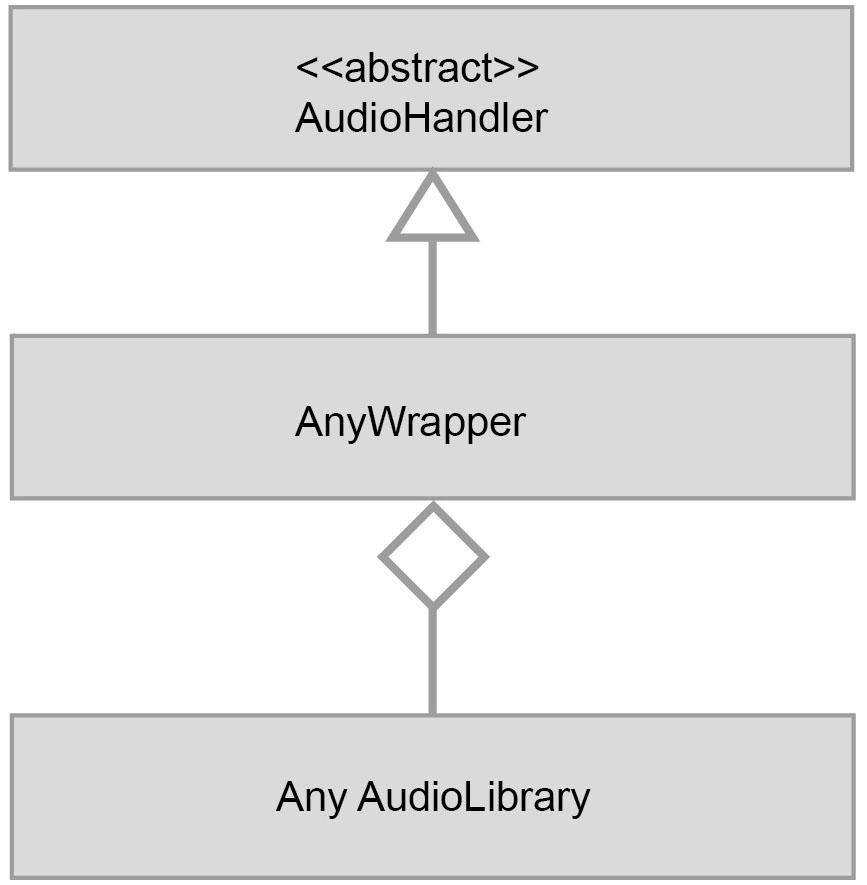
\includegraphics[width=.45\textwidth]{../img/AudioHandlerAnySimple}
\caption{UML-Klassendiagramm des AudioHandlers}
\label{Fig:AudioHandlerAnySimple}
\end{figure}

\FloatBarrier
\subsection{Verarbeitungskette}
\label{processingChain}

Die Klasse \texttt{AudioHandler} bietet eine Schnittstelle zur Hardware an. Ein Teil ihrer Implementierung ist die Verarbeitungskette. Durch ihr können andere Klassen mit den Audiodaten arbeiten, ohne die Implementierungsdetails des \texttt{AudioHandlers} kennen zu müssen. Im folgenden Abschnitt wird erklärt wie diese funktioniert.

\FloatBarrier
\subsubsection{AudioProcessor}
Eine Klasse, die mit Audiodaten arbeiten will, muss das Interface \texttt{AudioProcessor} implementieren, siehe Abbildung \ref{Fig:AudioProcessorExample}. Hierfür muss sie die Methoden \texttt{process"-Input"-Data()} und \texttt{process"-Output"-Data()} implementieren. \texttt{process"-Input"-Data()} wird immer aufgerufen, wenn Audiodaten vom Mikrofon für die Verarbeitung im internen Buffer vorhanden sind. Wenn der zweite interne Buffer zum Abspielen von Audiodaten leer ist, wird die Methode \texttt{process"-Output"-Data()} aufgerufen. Dort können Daten auf den Buffer zum Abspielen hinterlegt werden. Beide Funktionen haben als Parameter den jeweiligen Buffer und die Größe des Buffers. Der Rückgabewert der Funktion ist die neue oder alte Größe des Buffers. Der Rückgabewert ist nur auf Hinblick des Dekodieren und Kodieren relevant.
\newline
\begin{figure}[htp]
\centering
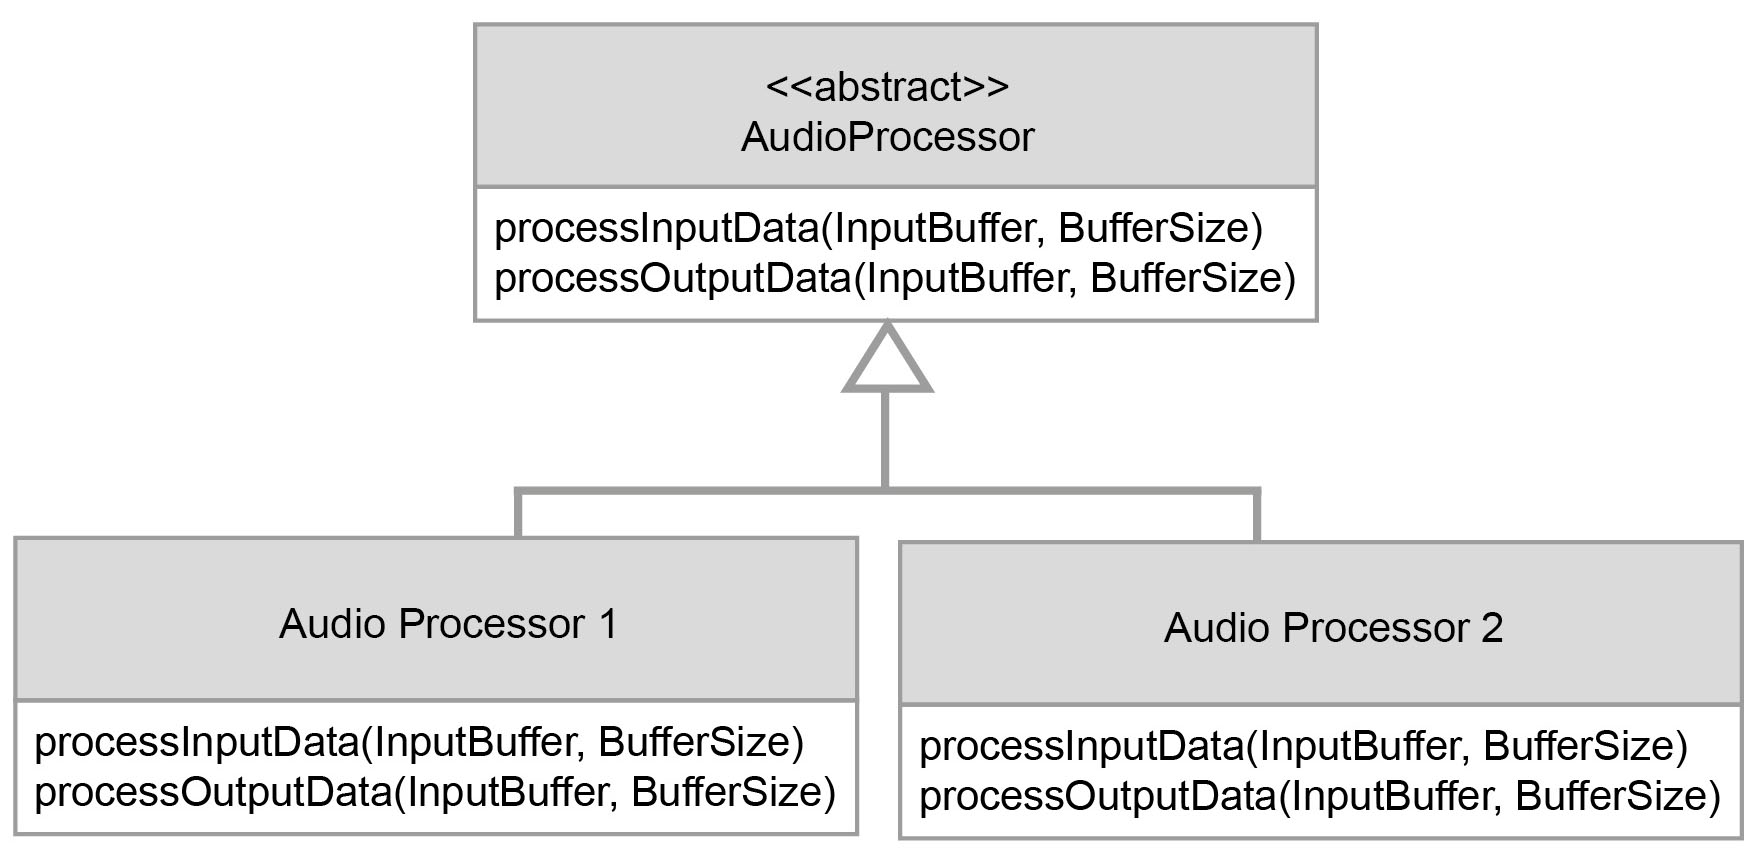
\includegraphics[width=1\textwidth]{../img/AudioProcessorExample}
\caption{Beispielhafte Verwendung der AudioProcessor-Klasse}
\label{Fig:AudioProcessorExample}
\end{figure}

\texttt{configure()} und \texttt{cleanUp()} sind weitere Methoden des AudioProcessors, die nicht in der Abbildung \ref{Fig:AudioProcessorExample} zu sehen sind. Erstere wird einmalig aufgerufen, kurz bevor die Verarbeitung gestartet wird. Als Parameter muss die festgelegte Audiokonfiguration übergeben werden. Die Funktion hat einen boolschen Rückgabewert der angibt, ob der AudioProcessor bereit für die Audioverarbeitung ist. Im Fehlerfall startet die Verarbeitung nicht. Dies kann wichtig sein, wenn z.B. ein \texttt{AudioProcessor} eine gewisse Audiokonfiguration voraussetzt. \texttt{cleanUp()} dient dazu, den \texttt{AudioProcessor} ordentlich aufzuräumen, wenn dieser nicht mehr benötigt wird.

\FloatBarrier
\subsubsection{Registrieren von Audioprozessoren}
Das Implementieren der Klasse \texttt{AudioProcessor} reicht nicht aus, um an der Audioverarbeitung aktiv teilzunehmen. Abbildung \ref{Fig:AudioHandlerAudioProcessor} zeigt die Beziehung zwischen \texttt{Audio"-Handler} und \texttt{Audio"-Processor}. Die Klasse muss sich beim \texttt{AudioHandler} mit der Methode \texttt{addProcessor()} anmelden. Diese nimmt als Parameter einen \texttt{AudioProcessor} entgegen. Audioprozessoren lassen sich über ihren Namen eindeutig identifizieren. Der Prozessor wird, falls er nicht schon vorhanden ist, in einer Liste vom Typ \texttt{AudioProcessor} eingefügt. Falls nun Audioinputdaten anliegen, so werden von allen Audioprozessoren, die sich in der Liste befinden, die \texttt{process"-Input"-Data()}-Methoden aufgerufen. Die Aufrufreihenfolge ist abhängig von der Anmeldereihenfolge. Für Audiooutput-Daten geschieht das analog, jedoch ist hier die Aufrufreihenfolge entgegengesetzt, da die Verarbeitungskette nicht kommutativ ist. Nur so ist es möglich an die ursprünglichen Audiodaten zu gelangen. Das Konzept hat einige Vorteile, z.B. können sich beliebige viele Prozessoren beim \texttt{AudioHandler} anmelden, jedoch ist hierbei der Aspekt der Performanz zu berücksichtigen. Des weiteren können Audioprozessoren zur Laufzeit hinzugefügt werden und beeinflussen sich nicht gegenseitig. Änderungen am \texttt{AudioHandler} sind ebenfalls unabhängig von den Prozessoren.
Vom Aufbau ähnelt die Verarbeitungskette dem Observer-Pattern, jedoch mit dem entscheidenden Unterschied, dass die Einfügereihenfolge eine wesentliche Rolle für die Verarbeitung spielt. 
\newline
\begin{figure}[htp]
\centering
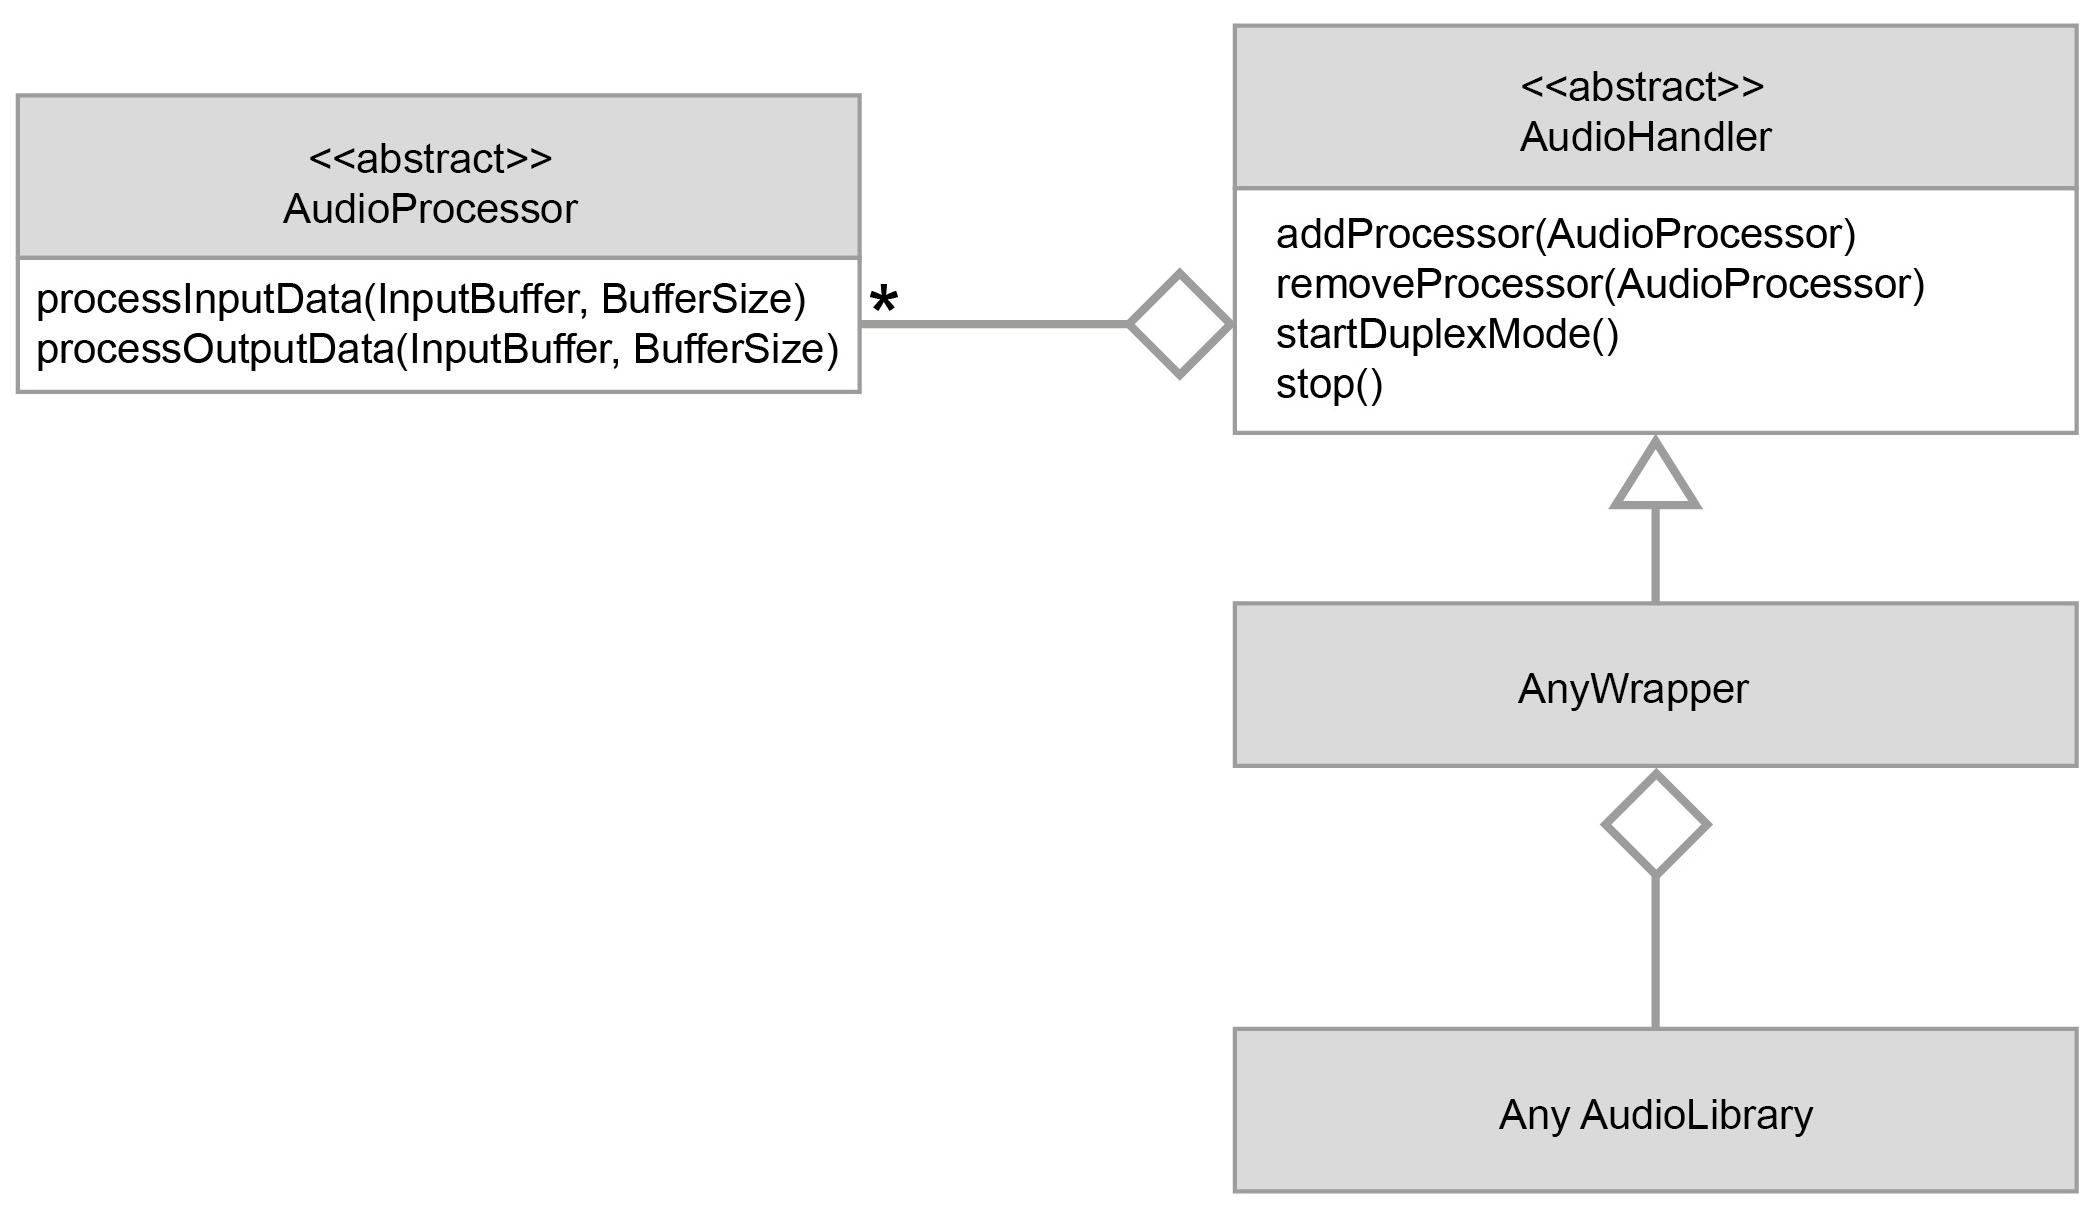
\includegraphics[width=1\textwidth]{../img/AudioHandlerAudioProcessor}
\caption{UML-Klassendiagramm AudioHandler und AudioProcessors}
\label{Fig:AudioHandlerAudioProcessor}
\end{figure}

\FloatBarrier




\subsubsection{ProfilingAudioProcessor}
Beim \texttt{Profiling"-AudioProcessor} handelt es sich um eine spezielle Unterklasse des \texttt{AudioProcessors}, siehe Abbildung \ref{Fig:ProfilingAudioProcessor}. Der Prozessor hat die Aufgabe, Anforderung \ref{FA:Statistik} umzusetzen. Die Umsetzung erfolgt mit dem Decorator-Pattern. Dieses ermöglicht es ein Objekt dynamisch zur Laufzeit zu erweitern. Der \texttt{Profiling"-AudioProcessor} ist dabei zum einem Unterklasse des zu erweiterten Objekt und zum anderen hat es eine Referenz darauf. Der Konstruktor des \texttt{Profiling"-AudioProcessor} nimmt als Parameter einen Pointer vom Typ \texttt{AudioProcessor} entgegen und speichert die Referenz. Der \texttt{Profiling"-AudioProcessor} muss die Methoden der Oberklasse implementieren, jedoch werden deren Aufrufe an die gespeicherte Referenz des \texttt{AudioProcessors} weitergeleitet. Funktionen die erweitert werden sollen, können vor und nach der Delegation ergänzt werden.
\newline
\begin{figure}[htp]
\centering
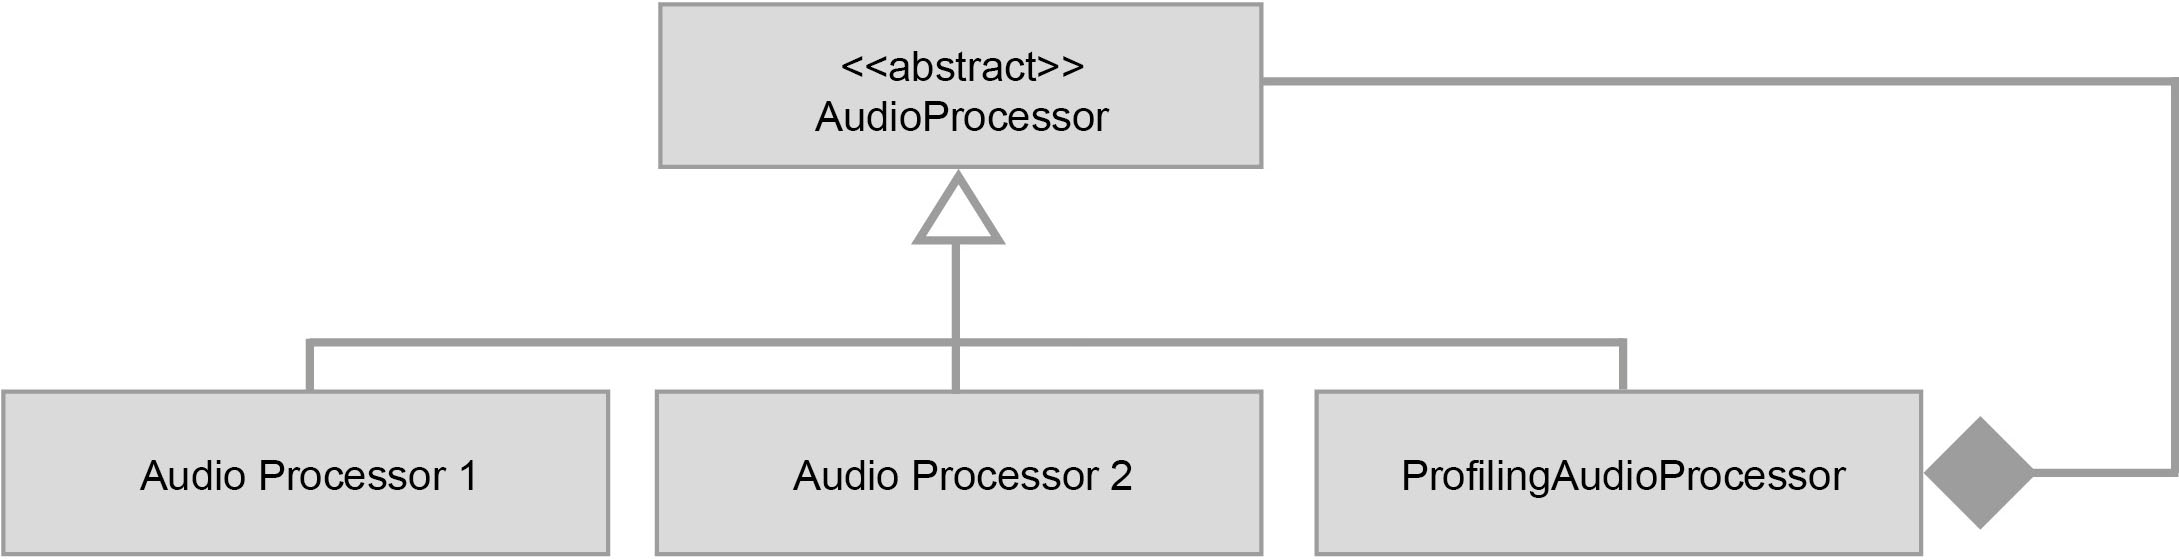
\includegraphics[width=1\textwidth]{../img/ProfilingAudioProcessor}
\caption{UML-Klassendiagramm des ProfilingAudioProcessors}
\label{Fig:ProfilingAudioProcessor}
\end{figure}

\FloatBarrier

\subsection{Austauschbarkeit und Instantiierung}
Um der Anforderung \ref{NFA:Softwarearchitektur} gerecht zu werden und die Komponenten austauschbar zu halten, wird das Entwurfsprinzip \texttt{Program to an interface, not to an implementation} \cite{Lahres2009}[Kap. 3.5] umgesetzt. Dies ermöglicht eine höhere Flexibilität, da der abstrakte Typ zur Laufzeit durch ein konkretes Objekt ausgetauscht werden kann. In diesem Zusammenhang bietet es sich an das Factory-Method-Pattern zu integrieren. Dabei wird die Instantiierung in einer Fabrikmethode ausgelagert. Als Parameter erwartet die Funktion ein String mit dem Namen der zu instantiierten Klasse. Alle Klassen basieren auf den gemeinsamen abstrakten Basistypen, der auch gleichzeitig Rückgabetyp ist. Die Fabrikmethoden wurde in eigenen Fabrikklassen ausgelagert, wie in Abbildung \ref{Fig:Factories} zu sehen ist. \texttt{getAudioHandler()} und \texttt{getAudioProcessor()} stellen die Fabrikmethoden dar. \texttt{getAudioHandlerNames()} und \texttt{getAudioProcessorNames()} liefern die Namen der Klassen, die instantiierbar sind.
\newline
\begin{figure}[htp]
\centering
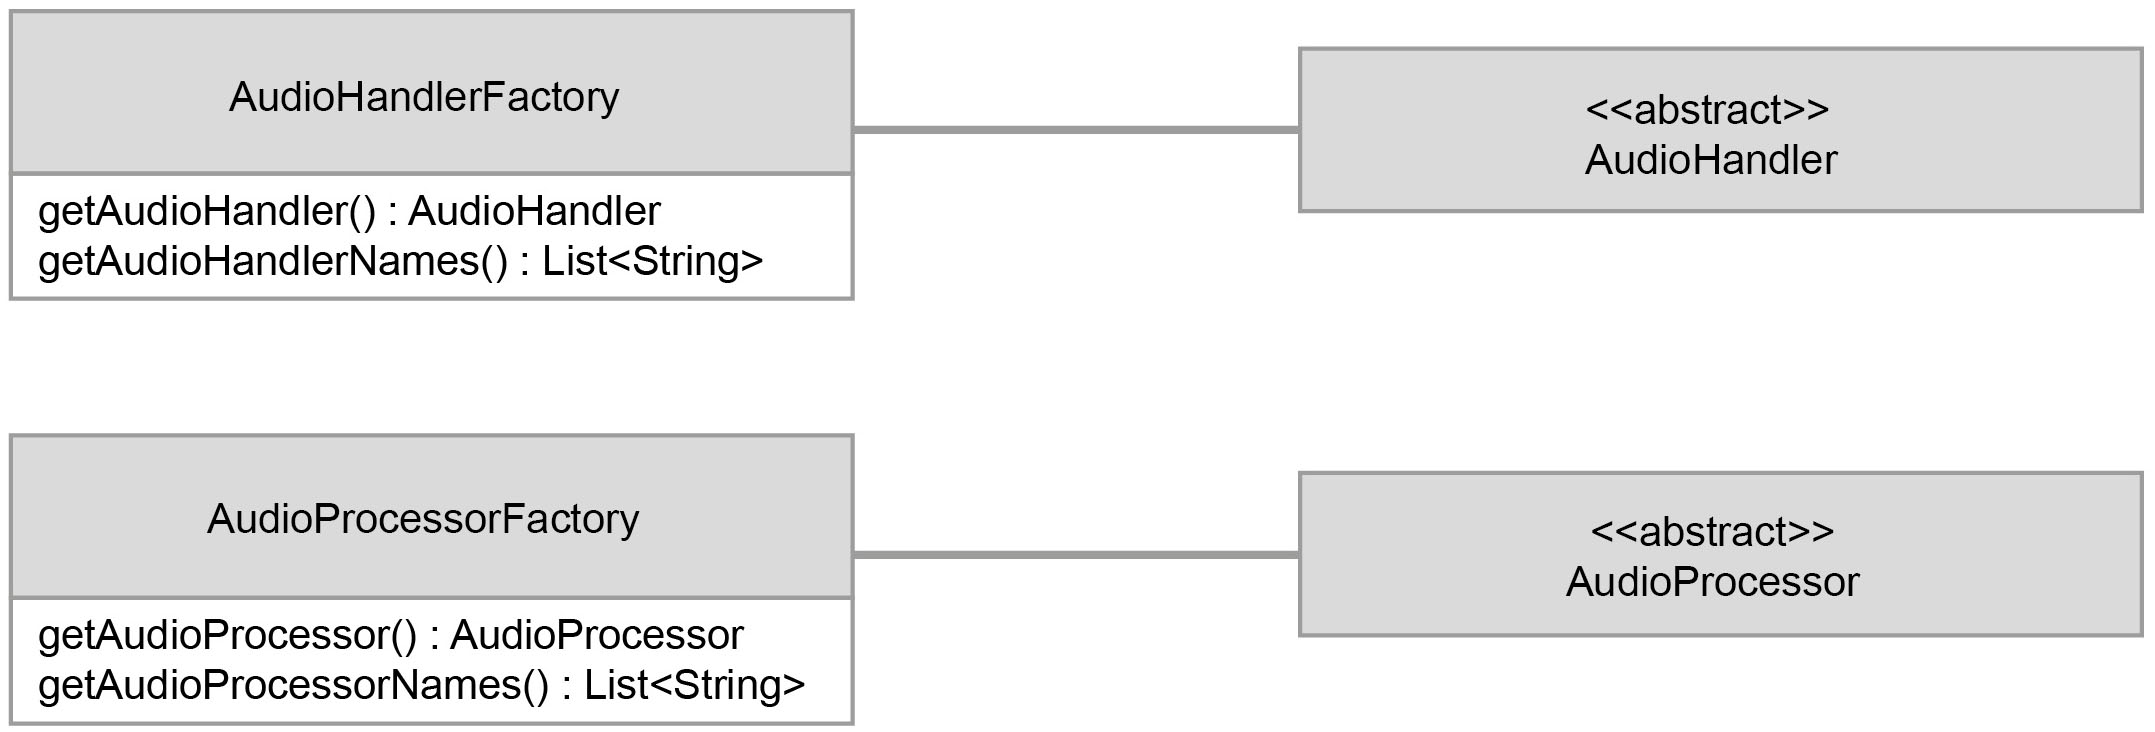
\includegraphics[width=1\textwidth]{../img/Factories}
\caption{Factory-Klassen im Überblick}
\label{Fig:Factories}
\end{figure}

\FloatBarrier

\subsection{RTP-Protokoll}
\label{rtp}
Das Real-time Transport Protocol (RTP) ist ein Netzwerkprotokoll für die Übertragung von Echtzeitdaten, wie Audio- und Videostreams oder -Konversationen, ist im RFC 3550 der Internet Engineering Task Force (IETF) definiert (siehe \cite{RFC3550}) und unterstützt sowohl Unicast- als auch Multicast-Sitzungen. RTP ist ein Protokoll für die Anwendungsebene und kann auf beliebigen Transportprotokollen wie UDP oder TCP aufgesetzt werden. Jedoch wird RTP meist mit UDP verwendet, da aufgrund der Echtzeitvoraussetzungen der Verlust von Paketen erträglicher ist als das Blockieren weiterer Daten durch erneutes Senden nicht-angekommener Pakete, so wie es in TCP üblich ist. Dies hat wiederum zur Folge, dass eine auf RTP mit UDP basierende Anwendung den Verlust einzelner Pakete kompensieren muss. Ein RTP-Paket besteht aus dem RTP-Header und dem anwendungsspezifischen Payload (Body). Der RTP-Header hat eine Größe von zwölf bis 72 Bytes und definiert folgende Felder:
\begin{lstlisting}[keepspaces=true,numbers=none,label=lst=rtpHeader,caption=RTP Header \cite{RFC3550}]
 0                   1                   2                   3
 0 1 2 3 4 5 6 7 8 9 0 1 2 3 4 5 6 7 8 9 0 1 2 3 4 5 6 7 8 9 0 1
+-+-+-+-+-+-+-+-+-+-+-+-+-+-+-+-+-+-+-+-+-+-+-+-+-+-+-+-+-+-+-+-+
|V=2|P|X|  CC   |M|     PT      |       sequence number         |
+-+-+-+-+-+-+-+-+-+-+-+-+-+-+-+-+-+-+-+-+-+-+-+-+-+-+-+-+-+-+-+-+
|                           timestamp                           |
+-+-+-+-+-+-+-+-+-+-+-+-+-+-+-+-+-+-+-+-+-+-+-+-+-+-+-+-+-+-+-+-+
|           synchronization source (SSRC) identifier            |
+=+=+=+=+=+=+=+=+=+=+=+=+=+=+=+=+=+=+=+=+=+=+=+=+=+=+=+=+=+=+=+=+
|            contributing source (CSRC) identifiers             |
|                             ....                              |
+-+-+-+-+-+-+-+-+-+-+-+-+-+-+-+-+-+-+-+-+-+-+-+-+-+-+-+-+-+-+-+-+
\end{lstlisting}
\begin{description}
\item[Version:] Hat in RFC 3550 immer den Wert 2, frühere Versionen hatten den Wert 1.
\item[Padding-Bit:] Gibt an, ob die Daten des RTP-Pakets auf ein Vielfaches von 4 Byte gepadded sind.
\item[Extension-Bit:] Gibt an, ob eine RTP Header-Extension existiert, die direkt an den Header anschließt.
\item[CSRC Count:] Gibt die Anzahl der Contribution Sources (CSRCs) an, maximal 15 aufgrund der Größe des Feldes mit 4 Bit.
\item[Marker-Bit:] Anwendungsspezifische Bedeutung.
\item[Payloadtype:] Gibt den Typ der transportierten Daten an. Dieser kann aus einer Liste vordefinierter Typen aus RFC 3551 oder dynamisch ausgewählt sein.
\item[Sequence number:] Gibt die Position des RTP-Pakets innerhalb des Datenstroms an und wird für die Umsortierung der Pakete verwendet. Der Anfangswert dieses Felds sollte zufällig gewählt werden.
\item[Timestamp:] Zeitpunkt, zu dem das erste Byte des Pakets erstellt wurde, wobei auch hier der Anfangswert zufällig gewählt wird.
\item[Synchronization Source Identifier:] Zufällig gewählte Zahl zum eindeutigen identifizieren des Senders dieses Pakets, auch SSRC genannt.
\item[Contribution Source Identifier:] Beinhaltet die originalen SSRCs der Teilpakete, wenn das Paket von einem Mixer aus verschiedenen Teilpaketen zusammengestellt wurde, werden auch CSRCs abgekürzt.
\end{description}
Im OHMComm-Framework wird RTP auf Basis von UDP verwendet, um den Verlust von Paketen zu Entdecken und eine Sortierreihenfolge festzulegen. Da OHMComm keine Sitzungen mit mehr als zwei Teilnehmern oder verschiedene Payload-Typen innerhalb einer Sitzung unterstützt, haben die meisten Header-Felder für das Framework keine Bedeutung. Jedoch werden für gesendete RTP-Pakete alle Header-Felder richtig belegt, um eine Interoperabilität mit anderen VoIP-Programmen zu gewährleisten. Für das Auslesen und Erstellen von RTP-Paketen sowie generieren der richtigen Header-Felder ist die Klasse \texttt{RTPPackageHandler} verantwortlich. So könnte man z.B. mithilfe von OHMComm eine  Sitzung mit mehreren Teilnehmern aufbauen, indem der lokale Client mit einem RTP-Mixer kommuniziert, der die Pakete dann auf die anderen Teilnehmer verteilt und auch deren Pakete vereint.
\subsubsection{RTCP-Protokoll}
\label{rtcp}
Das Real-time Transport Control Protocol (RTCP) ist auch in RFC 3550 definiert und bietet Möglichkeiten, Flusskontrolle für eine RTP-Sitzung durchzuführen sowie statistische Daten über die Verbindungsqualität (oder Quality of Service, kurz: QoS) zu übertragen. Ebenso werden Pakettypen für anwendungsspezifische Daten und zum Beenden einer RTP-Sitzung bereitgestellt. Im Gegensatz zu RTP-Paketen beinhalten RTCP-Pakete keine Daten, sondern bestehen nur aus RTCP-Headern. Jedoch ist in RFC 3550 vorgegeben, dass ein RTCP-Header nie einzeln, sondern nur in Gruppen von mindestens zwei Headern, sogenannten \enquote{compound packages}, versendet wird. Die verschiedenen RTCP-Pakettypen bestehen aus den ersten acht Bytes, die für alle Typen die gleiche Bedeutung haben, sowie einen Typ-spezifischen Teil. Der gemeinsame Header-Teil besteht aus den folgenden Feldern:
\\
\begin{lstlisting}[keepspaces=true,numbers=none,label=lst=rtcpHeader,caption=RTCP Header \cite{RFC3550}]
 0                   1                   2                   3
 0 1 2 3 4 5 6 7 8 9 0 1 2 3 4 5 6 7 8 9 0 1 2 3 4 5 6 7 8 9 0 1
+-+-+-+-+-+-+-+-+-+-+-+-+-+-+-+-+-+-+-+-+-+-+-+-+-+-+-+-+-+-+-+-+
|V=2|P|    RC   |      PT       |             length            |
+-+-+-+-+-+-+-+-+-+-+-+-+-+-+-+-+-+-+-+-+-+-+-+-+-+-+-+-+-+-+-+-+
|                     SSRC of packet sender                     |
+=+=+=+=+=+=+=+=+=+=+=+=+=+=+=+=+=+=+=+=+=+=+=+=+=+=+=+=+=+=+=+=+
\end{lstlisting}
\begin{description}
\item[Version:] Hat in RFC 3550 immer den Wert 2, frühere Versionen hatten den Wert 1.
\item[Padding-Bit:] Gibt an, ob der RTCP-Header auf ein Vielfaches von 4 Byte gepadded ist. Padding darf nur das letzte Teilpaket eines zusammengesetzten Pakets angewendet werden.
\item[Item Count:] Gibt die Anzahl der Einträge in diesem RTCP-Header an. Die Bedeutung hiervon ist abhängig vom Pakettyp
\item[Package Type:] Gibt den Typ des RTCP-Paketes an
\item[length:] Die Länge des RTCP-Teilheaders in 32-Bit Blöcken, minus 1 (den ersten 32-Bit Block)
\item[SSRC:] Source Description des Senders, stimmt mit der SSRC von RTP-Paketen dieses Senders überein
\end{description}
RFC 3550 definiert folgende RTCP Pakettypen und deren Inhalten:
\begin{description}
\item[Sender Report:] Beinhaltet Informationen über die Anzahl an gesendeten Paketen und Daten eines Senders. Ebenso werden pro Teilnehmer, von dem der Sender des Sender Reports Pakete empfangen hat, Daten über die Quality of Service (Anzahl verlorener Paketen, Netzwerkjitter, letzter empfangener Sender Report) verschickt. Diese Reception Report genannten Blöcke ermöglichen, dass jeder Teilnehmer einer RTP-Sitzung von jedem anderen Teilnehmer in regelmäßigen Abständen Feedback über die Übertragungsqualität bekommt. Jeder aktive Sender in einer RTP-Sitzung muss alle zusammengesetzten RTCP-Pakete immer mit einem Sender Report beginnen.
\item[Receiver Report:] Äquivalent zum Sender Report für passive Teilnehmer (also Teilnehmer die selbst keine Daten verschicken). Beinhaltet keine Informationen zur Anzahl verschickter Daten, aber trotzdem die Liste der Reception Reports für alle anderen Sender. Jeder passive RTP-Teilnehmer muss ein zusammengesetztes Paket immer mit einem Receiver Report beginnen.
\item[Source Description:] Beinhaltet eine Liste an informativer Daten über den Teilnehmer mit der angegebenen SSRC. Diese Daten, wie Telefonnummer, E-Mail, Webseite und Name können von Client-Programmen für die anderen Teilnehmer einer Sitzung angezeigt werden.
\item[BYE:] Der BYE RTCP-Header benachrichtigt die Teilnehmer einer Sitzung, dass der Sender mit der angegebenen SSRC die Sitzung verlässt und muss immer als letztes Paket eines zusammengesetzten Pakets stehen.
\item[Application-defined:] Der letzte Pakettyp bietet die Möglichkeit, anwendungsspezifische Daten zu übertragen. Dafür wird ein Name zur Identifikation des Typs der Daten und ein variabel großer Block für die eigentlichen Daten bereitgestellt.
\end{description}
Im OHMComm-Framework werden RTCP-Pakete in der Klasse \texttt{RTCPPackage\-Handler} erstellt sowie ausgelesen und in \texttt{RTCPHandler} verschickt und empfangen. \texttt{RTCPHandler} besitzt einen eigenen Thread, der auf einem dedizierten RTCP-Port auf ankommende Pakete wartet sowie in regelmäßigen Abständen (oder wenn explizit dazu aufgefordert) RTCP-Pakete verschickt. Folgende Pakettypen werden von der RTCP-Implementierung verwendet:
\\
In regelmäßigen Abständen wird ein zusammengesetztes Paket aus \textbf{Sender Report} (mit einem Reception Report) und \textbf{Source Description} versendet, wie es RFC 3550 vorschreibt. Jede empfangenen Sender Report oder Source Description Pakete werden in der prototypischen Anwendung derzeit nicht weiter verarbeitet, sondern nur auf der Konsole ausgegeben. Wenn die OHMComm-Anwendung beendet wird, wird zu den beiden genannten Pakettypen ein \textbf{BYE}-Paket angehängt, das auf der Empfänger-Seite dafür sorgt, dass die Kommunikation auch dort ordnungsgemäß abgebaut wird. Somit wird beim Beenden eines der Klienten der andere auch beendet, zumindest für die Kommunikation zwischen zwei OHMComm-Frameworks. Zusätzlich wird für die \textbf{passive Konfiguration} aus Abschnitt \ref{configurationUsages} der \textbf{Application-defined} Pakettyp verwendet, um eine Konfigurationsanfrage zu stellen und die geteilten Einstellungen auszutauschen. Der genaue Ablauf der passiven Konfiguration wird in Abschnitt \ref{passiveConfiguration} beschrieben.

\subsection{Jitter-Buffer}
\label{jitterBuffer}
Wie bereits in Abschnitt \ref{rtp} erwähnt, wird eine Echtzeitübertragung mit RTP meist mit dem Transportprotokoll UDP verwendet. Da UDP aber nicht garantiert, dass versendete Pakete beim Empfänger ankommen und auch nicht, in welcher Reihenfolge, muss die Anwendung dafür sorgen, dass mit verlorenen Paketen oder Paketen, die in der falschen Reihenfolge empfangen werden, richtig umgegangen wird. Dafür gibt es auf der Empfängerseite einen Jitter-Buffer, einen Puffer, der empfangene Pakete speichert und aus dem die weitere Prozessorkette Pakete in der richtigen Reihenfolge auslesen kann. Der Begriff Jitter-Buffer kommt von dem englischen Wort Jitter, dass für die Netzwerkverzögerung, -- oder genauer: die Varianz der Netzwerkverzögerung -- steht. Wie der Name schon andeutet, ist es eine der Aufgaben eines Jitter-Buffers, die Verzögerung des Netzwerkes und deren Schwankung auszugleichen. Ebenso sortiert ein Jitter-Buffer die empfangenen Pakete anhand ihrer RTP Sequenz-Nummer um und kaschiert den Verlust von Paketen. Bei Bibliotheken oder Programmen, die Sitzungen mit mehreren Teilnehmern unterstützen -- was bei OHMComm nicht der Fall ist -- muss für jeden anderen Sender ein eigener Jitter-Buffer verwaltet werden, da die Pakete der verschiedenen Sender verschiedene Netzwerkverzögerungen aufweisen können.
\\
Bei der Netzwerkübertragung über UDP können Pakete verloren gehen, oder sie werden so spät empfangen, dass sie bereits hätten abgespielt werden müssen, sog. \enquote{late loss}. Um den Audiotreiber trotzdem Daten zum Abspielen zu liefern, und nicht die Ausgabe ins Stocken zu bringen, muss ein Echtzeitkommunikationsprogramm dafür sorgen, dass diese Verluste von Audiodaten ausgeglichen werden. Diese Funktion nennt sich \enquote{loss concealment} (also: Verstecken von Verlusten) und kann auf verschiedene Arten umgesetzt werden. Die einfachste Möglichkeit ist es, wenn ein Paket angefordert wird, dass (noch) nicht empfangen worden ist, die Audiodaten dieses Pakets mit \textbf{Stille} zu ersetzen. Stille lässt sich sehr einfach erzeugen (z.B: durch Setzen aller Samples auf Null), ist ab einer gewissen Dauer für den Menschen hörbar und unterbricht den Fluss des Gesprächs, das Gespräch kling abgehakt. Als weitere Möglichkeit kann anstatt der Stille ein zufällig generiertes leises Rauschen, sog. \enquote{\textbf{comfort noise}}, abgespielt werden. Im Gegensatz zur absoluten Stille bekommt man bei Rauschen nicht so schnell das Gefühl, dass die Verbindung abgebrochen ist. Eine dritte Möglichkeit wiederholt das letzte erfolgreich empfangene Paket und spielt es erneut ab. Da sich der Tonverlauf der menschlichen Stimme nicht so schnell ändert, %TODO ca. Zeitdauer
besteht eine große Wahrscheinlichkeit, dass die Audiodaten des verlorene Pakets dem vorherigen sehr ähnlich sind und der Unterschied kaum hörbar wird. Alle drei dieser einfachen Methoden für \enquote{loss concealment} sind einfach zu implementieren und besitzen eine geringe Laufzeit, werden dafür vor Allem bei längeren Stille-Perioden sehr schnell hörbar und stören den Gesprächsverlauf. Deshalb gibt es noch eine Vielzahl weiterer Algorithmen, die versuchen, Unterbrechungen möglichst unhörbar zu überdecken, dies jedoch meist auf Kosten erhöhter Laufzeit und Komplexität erkaufen.
\\
Um den Verlust von Paketen aufgrund von \enquote{late loss} gering zu halten und somit eine flüssige und möglichst vollständige Audiokommunikation zu gewährleisten, führt ein Jitter-Buffer eine künstliche Verzögerung zwischen dem Empfangen und dem Abspielen eines Paketes ein. Dadurch, dass ein Paket später abgespielt wird (der sog. \enquote{playout point} wird nach Hinten verschoben), hat es länger Zeit, beim Empfänger anzukommen, wodurch weniger Pakete wegen \enquote{late loss}, also dem Ankommen nach ihrem \enquote{playout point}, verworfen werden. Hierfür sollte die Abspielverzögerung so gewählt werden, dass möglichst alle Pakete, die nicht auf dem Netzwerk verloren gehen, den Empfänger vor ihrem Abspielzeitpunkt erreichen. Auf der anderen Seite darf die Abspielverzögerung nicht zu groß werden, sonst leidet die Qualität der Echtzeitkommunikation. Dafür wird in umfangreicheren Implementierungen die Abspielverzögerung meist dynamisch angepasst. Diese sog. \enquote{playout point adaption} wird auf Basis des Anteils an \enquote{late loss} berechnet und in bestimmten Abständen durch einschieben eines zusätzlichen Pakets (z.B. Stille) oder überspringen eines empfangenen Paketes umgesetzt. Der Jitter-Buffer des OHMComm-Frameworks heißt \texttt{RTPBuffer} und besitzt in der aktuellen Version eine feste Abspielverzögerung, die bei der Kompilierung des Programms eingestellt werden muss.
\\
Um ein asynchrones Empfangen von RTP-Paketen zu ermöglichen, wird der RTP-Listener (siehe Abschnitt \ref{rtpListener}) in einem eigenen Thread umgesetzt. Der RTP-Buffer oder Jitter-Buffer bietet die Schnittstelle zwischen dem Listener-Thread zum Empfangen von RTP-Paketen und der Verarbeitungskette, die die darin enthaltenen Audiodaten weiter behandelt. Dafür muss der Jitter-Buffer thread-safe implementiert sein, also gegen Data Races in den Puffereinträgen und anderen Werten abgesichert sein.
\\
Des Weiteren muss der Jitter-Buffer -- wie auch jede andere Komponente in der Verarbeitungskette -- performant umgesetzt werden, da jede Verzögerung in einer der Glieder der Verarbeitungskette die gesamte Aufnahme- oder Abspielverzögerung vergrößert, wodurch sich die Gesprächsqualität verschlechtert. Dafür wird der Jitter-Buffer -- so wie viele performance-kritische Puffer -- als Ringpuffer implementiert. Ein Ringpuffer ist als Array auf dem Speicher angelegt. Indem der Lese- oder Schreibindex am Ende des Arrays umgeschlagen wird (\texttt{modulo Buffergröße}), kann der Puffer als endlose Datenstruktur verwendet werden, die jedoch nur die letzten \texttt{x} Einträge besitzen kann (wobei \texttt{x} die Größe des Puffers ist). Dies stellt für den Jitter-Buffer keine Beeinträchtigung dar, da sowieso alle Pakete, die bereits gelesen worden sind, nicht mehr gebraucht werden und somit ein RTP-Buffer nur eine Hand voll neue Pakete halten muss. Die Vorteile eines Ringpuffers bestehen aus einem konstanten Speicherverbrauch im Gegensatz zu den vielen Allokationen und Deallokationen, die z.B. eine verkettete Liste benötigen würde, beim Hinzufügen und Entfernen von Paketen.
\subsection{Netzwerkverbindung}
Wie auch die meisten anderen Komponenten des OHMComm-Framework (Audio-Bibliothek, -Prozessoren) ist auch die Umsetzung der Netzwerkschnittstelle austauschbar implementiert. Dies wird durch die abstrakte Basisklasse \texttt{NetworkWrap\-per} umgesetzt, die Methodensignaturen zum Senden und Empfangen von Daten sowie zum Schließen der Verbindung bereitstellt. Bei einer Implementierung einer Netzwerkschnittstelle muss dafür gesorgt werden, dass die Senden- und Empfangen-Methoden keine Data-Races erzeugen können, da diese eventuell aus verschiedenen Threads heraus aufgerufen werden. Da RTP in den allermeisten Fällen mit dem Transportprotokoll UDP verwendet wird, gibt es jedoch derzeit nur eine konkrete Implementierung der Netzwerkschnittstelle namens \texttt{UDPWrapper}, die RTP-Pakete in UDP-Pakete verpackt und beim Empfangen wieder entpackt. Spätere Versionen des Frameworks enthalten zusätzlich noch eine Implementierung, die TCP verwendet.

\FloatBarrier
\subsection{RTPListener}
\label{rtpListener}
Die Socketmethoden zum Empfangen von Paketen sind blockierend \cite{WinsockReference}. Dies hat weitreichende Folgen für die Architektur. Der Ausgangspunkt der Verarbeitung ist die Verarbeitungskette im \texttt{Audio"-Handler}. Wird dort eine blockierende Funktion aufgerufen, so wird die gesamte Weiterverarbeitung blockiert. Wenn z.B. innerhalb eines Audioprozessors die blockierende Socket-Funktion \texttt{recv"-from()} aufgerufen wird, und es werden keine Pakete empfangen, dann bricht die gesamte Verarbeitung ab. Dieses Verhalten ist nicht erwünscht. Die Verarbeitung soll unabhängig von den empfangenen Paketen funktionieren. Die Klasse \texttt{RTPListener} stellt einen Lösungsansatz für dieses Problem dar. Hierfür wird der gesamte Empfangsprozess in einem eignen Thread ausgelagert. Abbildung \ref{Fig:RTPListenerAdvanced} zeigt den Aufbau des \texttt{RTPListeners}.
\newline
\begin{figure}[htp]
\centering
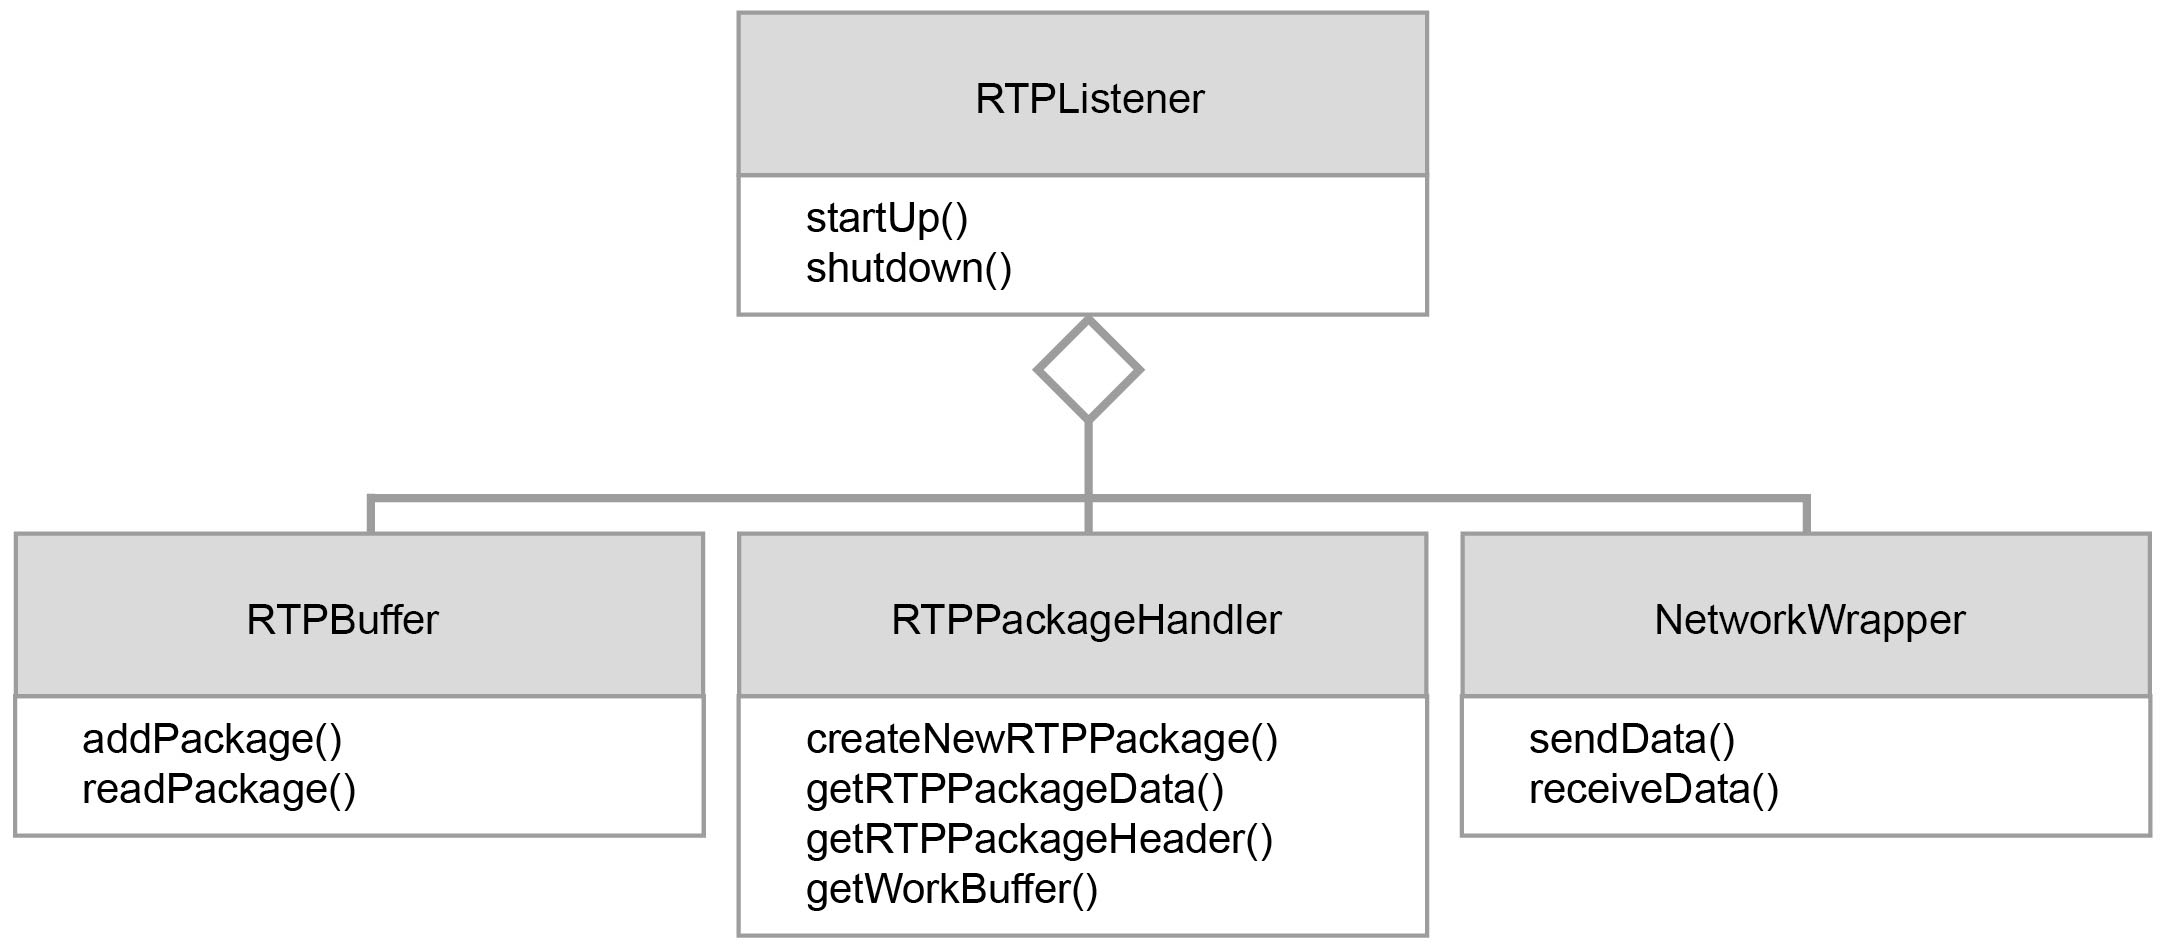
\includegraphics[width=1\textwidth]{../img/RTPListenerAdvanced}
\caption{Der gesamte Empfangsprozess in einem separaten Thread}
\label{Fig:RTPListenerAdvanced}
\end{figure}

Die Methode \texttt{startUp()} startet den \texttt{RTP"-Listener} in einem separaten Thread und \texttt{shut"-down()} beendet ihn wieder. Der Empfangsprozess besteht aus den Komponenten \texttt{RTP"-Buffer}, \texttt{RTP"-Package"-Handler} und dem \texttt{Network"-Wrapper}. Im Thread des \texttt{RTP"-Listeners} wird in einer Endlosschleife die blockierende Funktion \texttt{receive"-Data()} des \texttt{Network"-Wrappers} aufgerufen. Als Parameter wird der Funktion der Buffer des \texttt{RTP"-Package"-Handlers} übergeben. Hierfür wird die Funktion \texttt{getWork"-Buffer()} verwendet. Wenn ein Paket empfangen wurde, so kann mit Hilfe von \texttt{RTP"-Package"-Handler} der RTPHeader ausgelesen. Falls keine weitere Verarbeitung nötig ist, kann das Paket im \texttt{RTP"-Buffer} mit \texttt{add"-Package()} zwischengespeichert werden. Anschließend kann es mit \texttt{readPackage()} wieder ausgelesen werden. Das Auslesen des Paket erfolgt in der Regel vom Main-Thread, welches ohne Probleme möglich, da der \texttt{RTPBuffer} thread-safe ist (siehe Abschnitt \ref{jitterBuffer}).

\FloatBarrier

\section{Konkrete Softwarekomponenten}
\subsection{RtAudio}
\label{sec:RtAudio}
Als Audiowrapper wird RtAudio eingesetzt. RtAudio wird entwickelt von Gary P. Scavone, Professor an der McGill Uni in Kanada, und wird unter der MIT-Lizenz vertrieben. RtAudio dient als Programmierschnittstelle, engl. Application Programming Interface(API), zwischen den Betriebssystemabhängigen APIs und OHMComm. RtAudio unterstützt eine Vielzahl von APIs. Aufgeschlüsselt nach Betriebssystem sind diese:

\begin{description}
\item[Microsoft Windows:]~\par
\begin{itemize}
\item Audio Stream Input/Output (ASIO)
\item DirectSound
\item Windows Audio Session API (WASAPI)
\end{itemize}
\item[Mac OS X:]~\par
\begin{itemize}
\item CoreAudio
\item Jack Audio Connection Kit(Jack)
\end{itemize}
\item[GNU/Linux:]~\par
\begin{itemize}
\item Advanced Linux Sound Architecture (ALSA)
\item Open Sound System (OSS)
\item PulseAudio
\item Jack Audio Connection Kit(Jack)
\end{itemize} 
\end{description}

Ein alternativer plattformunabhängiger Audiowrapper wäre PortAudio, was jedoch in C geschrieben ist. Da OHMComm und RtAudio in C++ geschrieben sind, ist dies die bessere Kombination.

\subsection{Opus}

Als Audiocodec wird Opus eingesetzt. Opus ist ein Codec zur verlustbehafteten Kompression von Audiodaten. Opus ist speziell für Echtzeitanwendungen konzipiert und deshalb bestens geeignet für das OHMComm-Framework. Er wird unter einer OpenSource-Lizenz als royalty-free Codec, also ein Codec ohne Lizenzkosten, vertrieben. Alternative Codec wären AAC-LD oder AAC-ELD, welche aber Lizenzkostenpflichtig sind und deshalb nicht für OHMComm in Frage kommen. Opus ist ein Hybridcodec, welcher eine Transformationsschicht \textbf{CELT} als Nachfolger von Vorbis (Entwickelt von der Xiph.Org Foundation) und ein Linear Predictive Coding(LPC) namens \textbf{SILK} (Ursprünglich Entwickelt von Skype Technologies) zur Audiokompression einsetzt.

Viele bekannte Anwendungen setzten ebenfalls auf Opus als Audiocodec, darunter TeamSpeak, die Webbrowser Firefox und Chrome -- innerhalb ihrer WebRTC Implementierungen, da dort Opus vom Standard vorausgesetzt wird -- und Android 5 (Lollipop), welches eine native Unterstützung von Opus bietet.

Weitere Feature von Opus sind:

\begin{itemize}
\item Unterstütze Sampling Raten: 8000, 12000, 16000, 24000, und 48000Hz
\item 3 Application Modi:
\begin{itemize}
\item OPUS\_APPLICATION\_VOIP: Optimiert auf Sprachverständlichkeit
\item OPUS\_APPLICATION\_AUDIO: Optimiert auf Klanggenuss z.B. für Musik
\item OPUS\_APPLICATION\_RESTRICTED\_LOWDELAY: Optimiert auf kleinstmögliche Latenz
\end{itemize}
\item Audioframegrößen von 2.5 ms bis 60 ms
\item Mono und Stereo Support
\end{itemize}

\section{Statistiken}
Ein weiteres Feature des OHMComm-Frameworks ist das Sammeln und Anzeigen von statistischen Daten (siehe Anforderung \ref{FA:Statistik}). Die verschiedenen Statistiken wurden eingebaut, um die Performance einzelner Abschnitte der Verarbeitungskette zu messen, sowie die Richtigkeit der Handhabung von RTP-Paketen und frei gewählter Werte (wie der Buffergröße und Abspiellatenz) zu beweisen. Im Laufe des Programms werden eine Vielzahl an verschiedenen statistischen Daten gesammelt. Darunter fallen:
\begin{description}
\item[Audio-Daten:] Bei jedem Durchlauf der Verarbeitungskette werden Zähler für die Gesamtzahl der aufgenommenen sowie abgespielten Samples und Daten-Bytes erhöht.
\item[RTP-Daten:] Ebenso werden die Anzahl an versendeten und empfangenen RTP-Paketen, sowie die Größe deren Nutzdaten und der RTP-Header gezählt. Für das bestimmen der Quality of Service werden die Anzahl der verlorenen Pakete gezählt, sowie der maximale Füllstand des Jitter-Buffers gespeichert.
\item[Prozessor-Daten:] Wenn das messen der Prozessorlaufzeiten aktiviert ist, wird für jeden Audioprozessor in der Verarbeitungskette die Gesamtlaufzeit der beiden Methoden zum Bearbeiten der aufgenommenen oder abgespielten Daten gemessen.
\end{description}
Aus diesen gemessenen Werten werden beim Beenden des Frameworks verschiedene relevante Statistiken berechnet und ausgegeben. Die Ausgabe der Statistiken erfolgt immer über den Standardoutput (meist eine Konsole) sowie (falls vorher so konfiguriert) in eine Datei. Angezeigt werden die folgenden statistischen Werte:
\begin{itemize}
\item Die Gesamtzahl der aufgenommen und abgespielten Audiodaten (in Bytes) sowie Samples. Ebenso werden diese Werte durch die Gesamtlaufzeit der Kommunikation geteilt, um den Durchsatz der Soundkarte zu berechnen. An den Ergebnissen (vor allem an der Input- und Output-Samplerate) lässt sich erkennen, dass die Soundkarte sich nicht ganz an die vorher konfigurierte Samplerate hält, sondern leicht davon abweicht.
\item Die Gesamtzahl der gesendeten und empfangenen Daten (in Bytes) sowie Pakete. Wie auch im vorherigen Punkt sind hier die Durchsatz-Raten von größerer Bedeutung als die Gesamtzahlen. So wird hier der Datendurchsatz für die gesendeten und empfangene Pakete ausgerechnet, also die wirklich benötigte Netzwerkbandbreite in beide Richtungen. Ebenso werden die Bandbreiten der reinen Audiodaten und der prozentuale Overhead der RTP-Header ausgegeben. Der Header-Overhead ist abhängig von der Größe der Daten in einem RTP-Paket und liegt meist unter 5\%.
\item Die Anzahl der verlorenen Pakete (also nicht empfangene Sequenznummern, siehe Abschnitt \ref{rtp}) sowie der maximale Füllstand der Jitter-Buffers. Anhand dieser Werte kann die Übertragungsqualität sowie die maximale Abspielverzögerung (der maximale \enquote{playout point}) abgelesen werden. Für beide Werte gilt, je kleiner der Wert, desto besser ist die Qualität der Übertragung.
\item Aus der Gesamtmenge an aufgenommenen/abgespielten Audiodaten und der Gesamtmenge an gesendeten/empfangen Audiodaten lässt sich die Kommpres\-sions-/Dekompressionsrate berechnen, also wie stark ein verwendeter Audiocodec die Größe der Audiodaten komprimiert. Bei einer Kommunikation ohne zugeschalteten Audiocodec wird exakt die gleiche Anzahl an Bytes gesendet, die aufgenommen wird oder auch abgespielt, die empfangen wird, wodurch eine Kompression von 0\% angezeigt wird. Eine Verwendung des Opus-Codecs resultiert z.B. in einer Kompression von ca. 96\%, also werden nur 4\% der aufgenommen Audio-Bytes über das Netzwerk versendet und auch aus den empfangenen 4\% beim Entpacken wieder die volle Anzahl an Audiodaten wieder hergestellt. Daran kann man sehr gut die Bedeutung eines Audiocodecs für das Minimieren der benötigten Bandbreite erkennen.
\item Die Laufzeiten der verschiedenen Audioprozessoren. Wenn das Messen der Ausführungszeiten der Verarbeitungskette aktiviert wird, wird für jeden verwendeten Audioprozessor die Gesamtausführungszeiten der Methoden zum Bearbeiten des Audio-Inputs und -Outputs angezeigt. Auch hier wird zusätzlich der interessantere Wert der Ausführungszeit pro Aufruf ausgegeben, an dem die sog. algorithmische Verzögerung eines einzelnen Prozessors und der ganzen Verarbeitungskette abgelesen werden kann. Wenn die algorithmische Verzögerung der gesamten Prozessorkette zu groß wird, bekommt die Soundkarte nicht rechtzeitig neue Audiodaten und es wird ein hörbares Knacken ausgegeben.
\end{itemize}

\section{Dokumentation}
Für die Dokumentation wird das Tool Doxygen verwendet. Es unterstützt eine Vielzahl an Programmiersprachen und ist plattformunabhängig. Die Dokumentation des Quellcodes erfolgt im Quellcode selbst. Hier zu werden Kommentare mit besonderer Syntax verwendet, aus denen später die Dokumentation generiert werden kann. Dokumentationsformate sind HTML, RTF, PostScript, PDF oder Unix-Manpages. Es gibt unterschiedliche Stile für Dokumentationskommentare. OHMComm verwendet den QT-Style, da dieser häufig für C++ Projekte eingesetzt wird. Listing \ref{Code:QTstyle} zeigt wie eine solche Dokumentation im Quellcode aussehen kann. Kommentare zum Dokumentieren werden mit /*! eingeleitet. Die Parameter werden mit \/param und die Rückgabewerte mit \/return beschrieben. Doxygen erwartet, als Konsolenanwendung, einen Parameter mit den Einstellungen für die Dokumentation zum Generierien. Der Aufruf erfolgt mit \texttt{doxygen <config-file>}.

\begin{lstlisting}[caption={Code-Dokumentation im QT-Style},label={Code:QTstyle}, numbers=none]
	/*! Beschreibung der Methode
	 * $\@backslashchar{}$param a Parameterbeschreibung
	 * $\@backslashchar{}$param b Parameterbeschreibung
	 * $\@backslashchar{}$return Was wird zuckgegeben
	 */ 
	int testMe(int a, char *b);
\end{lstlisting}